\usetikzlibrary{shadows,arrows}
% Define the layers to draw the diagram
\pgfdeclarelayer{background}
\pgfdeclarelayer{foreground}
\pgfsetlayers{background,main,foreground}
 
% Define block styles  
\tikzstyle{rectangle}=[draw, fill=blue!20, text width=6.0em, text centered,
  minimum height=1.5em,drop shadow]
\tikzstyle{practica} = [rectangle, text width=8em, minimum width=10em,
  minimum height=3em, rounded corners, drop shadow]

\tikzstyle{circle}=[draw, fill=green!20, text width=6.0em, text centered,
  minimum height=1.5em,drop shadow]
\tikzstyle{interface} = [circle, text width=8em, minimum width=10em,
  minimum height=3em, rounded corners, drop shadow]
 
\tikzstyle{texto} = [above, text width=6em, text centered]
\tikzstyle{linepart} = [draw, thick, color=black!50, -latex', dashed]
\tikzstyle{line} = [draw, thick, color=black!50, -latex']
 
% Define distances for bordering

\newcommand{\practica}[3]{node (p#1) [practica] {#2 \\ \scriptsize\textit{#3}}}
\newcommand{\implemented}[3]{node (p#1) [interface] {#2 \\ \scriptsize\textit{#3}}}

% Draw background
\newcommand{\background}[5]{%
  \begin{pgfonlayer}{background}
    % Left-top corner of the background rectangle
    \path (#1.west |- #2.north)+(-0.5,0.5) node (a1) {};
    % Right-bottom corner of the background rectanle
    \path (#3.east |- #4.south)+(+0.5,-0.25) node (a2) {};
    % Draw the background
    \path[fill=yellow!20,rounded corners, draw=black!50, dashed]
      (a1) rectangle (a2);
    \path (a1.east |- a1.south)+(0.8,-0.3) node (u1)[texto]
      {\scriptsize\textit{#5}};
  \end{pgfonlayer}}

\newcommand{\transreceptor}[3]{%
  \path [linepart] (#1.east) -- node [above]
    {\scriptsize Transreceptor #2} (#3);}

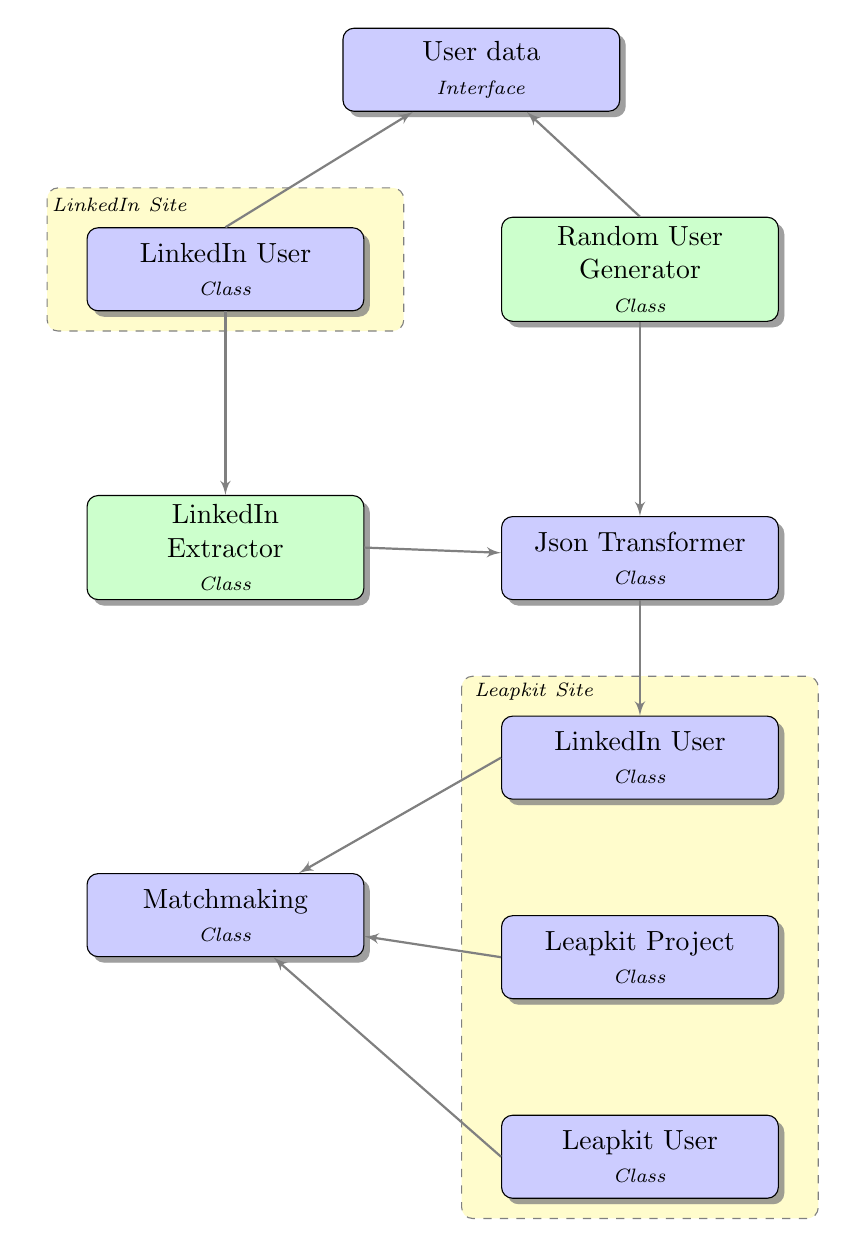
\begin{tikzpicture}


% Draw diagram elements
\path                        \practica{1}{User data}{Interface};
\path (p1.south)+(-3.25,-2.0) \practica{2}{LinkedIn User}{Class};
\path (p2.east) +( 3.5, 0.0) \implemented{3}{Random User Generator}{Class};

\path (p2.south) +( 0.0,-3.0) \implemented{4}{LinkedIn Extractor}{Class};
\path (p3.south) +( 0.0,-3.0) \practica{5}{Json Transformer}{Class};


\path (p5.south)+(0.0,-2.0) \practica{6}{LinkedIn User}{Class};
\path (p6.south)+(0.0,-2.0) \practica{7}{Leapkit Project}{Class};
\path (p7.south)+(0.0,-2.0) \practica{8}{Leapkit User}{Class};
 
\path (p4.south)+(0.0,-4.0) \practica{9}{Matchmaking}{Class};

% Draw arrows between elements
\path [line] (p2.north) -- node [above] {} (p1);
\path [line] (p3.north) -- node [above] {} (p1);

\path [line] (p2.south) -- node [above] {} (p4);
\path [line] (p3.south) -- node [above] {} (p5);

\path [line] (p4.east) -- node [above] {} (p5);

\path [line] (p5.south) -- node [above] {} (p6);
\path [line] (p6.west) -- node [above] {} (p9);
\path [line] (p7.west) -- node [above] {} (p9);
\path [line] (p8.west) -- node [above] {} (p9);

\background{p2}{p2}{p2}{p2}{LinkedIn Site}
\background{p6}{p6}{p8}{p8}{Leapkit Site}

\end{tikzpicture}
